\subsection{Lab4: Modulación ASK en GRC}

%*********************
\begin{frame}{}

\pgfdeclareimage[width=\paperwidth,height=\paperheight]{bg}{imagenes/fondo_lab}
\setbeamertemplate{background}{\pgfuseimage{bg}}

\bfseries{\textrm{\LARGE Lab4\\ \Large Modulación ASK en GRC}}
\raggedright
\end{frame}
%*********************

%--------------------------

\begin{frame}{Modulación ASK en GRC}


\pgfdeclareimage[width=\paperwidth,height=\paperheight]{bg}{imagenes/fondo3}
\setbeamertemplate{background}{\pgfuseimage{bg}}

  \begin{itemize}
  \item {
En esta práctica se hace uso de la  Modulación por desplazamiento de amplitud (ASK) este es un esquema de modulación digital en el que la amplitud de la onda portadora se cambia con respecto a la señal de información, manteniendo la fase y la frecuencia de constantes. Para el presente laboratorio, se utilizó BASK, el cual tiene el mismo comportamiento, pero utilizando bits. Donde su comportamiento es descrito por la siguiente ecuación:

\begin{equation*}
S(t) = Am(t)cos(wt)
\end{equation*}

  }
  \item {
El diagrama de bloques en GRC consiste en la multiplicación de una señal de información con una portadora, que corresponde a una señal coseno de diez veces la frecuencia de la información. La frecuencia de muestreo debe ser mayor que el doble de la frecuencia máxima de la señal de datos.
  }
  \end{itemize}
\end{frame}
%---------------------------

\begin{frame}{Modulación ASK en GRC}

\begin{figure}[H]
\centering
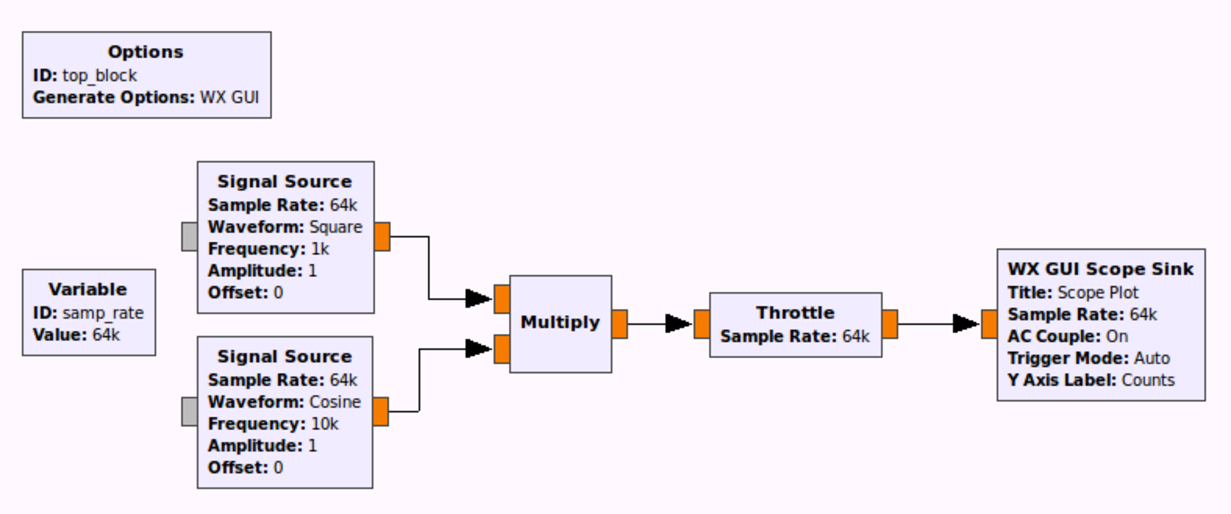
\includegraphics[width=\textwidth]{parte1/lab4/pdf/lab4_1.pdf}
\end{figure}
Diagrama de bloques en GNU radio, para generar una modulación ASK entre dos señales.
\end{frame}
%--------------------

\begin{frame}{Modulación ASK en GRC}
\vspace{-1cm}
\begin{figure}[H]
\centering
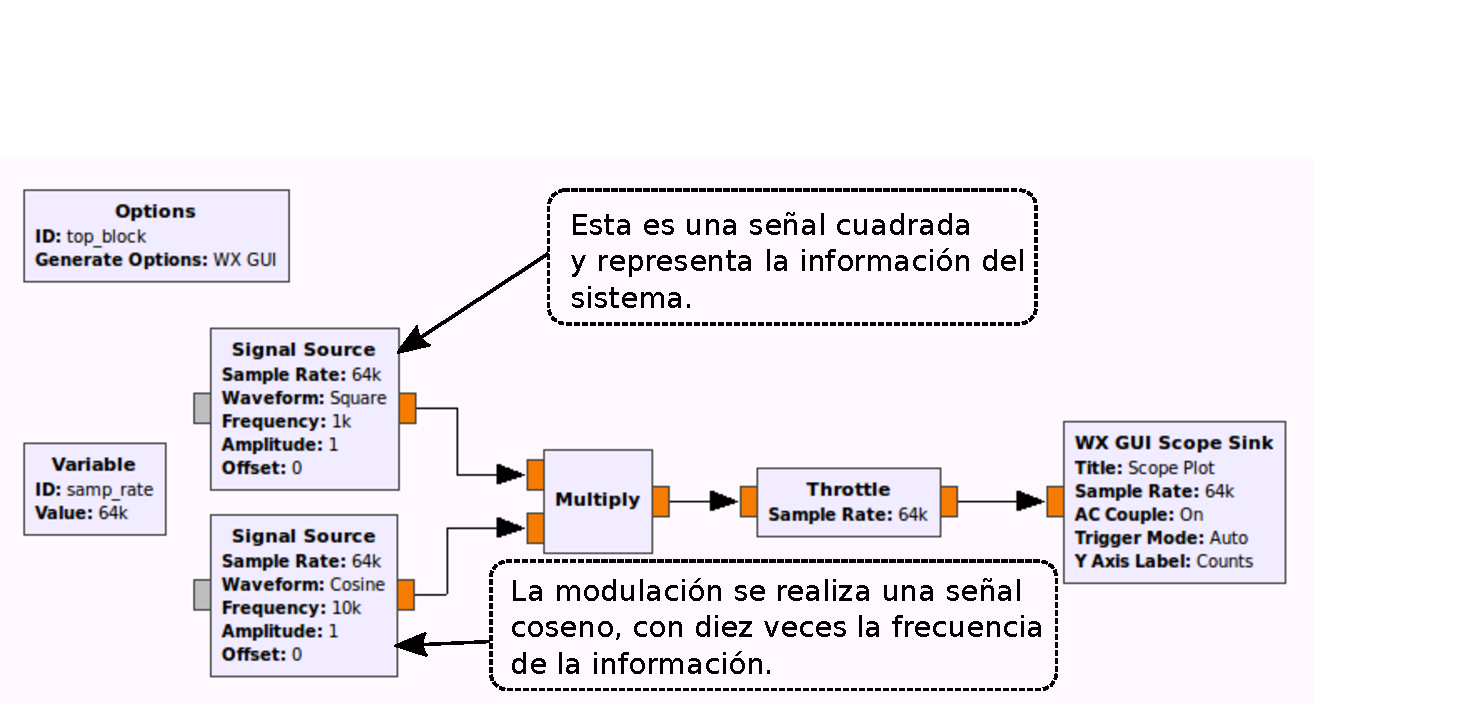
\includegraphics[width=1.1\textwidth]{parte1/lab4/pdf/lab4_2.pdf}
\end{figure}
\end{frame}
%_---------------------

\begin{frame}{Modulación ASK en GRC}
\vspace{-1.5cm}
\begin{figure}[H]
\centering
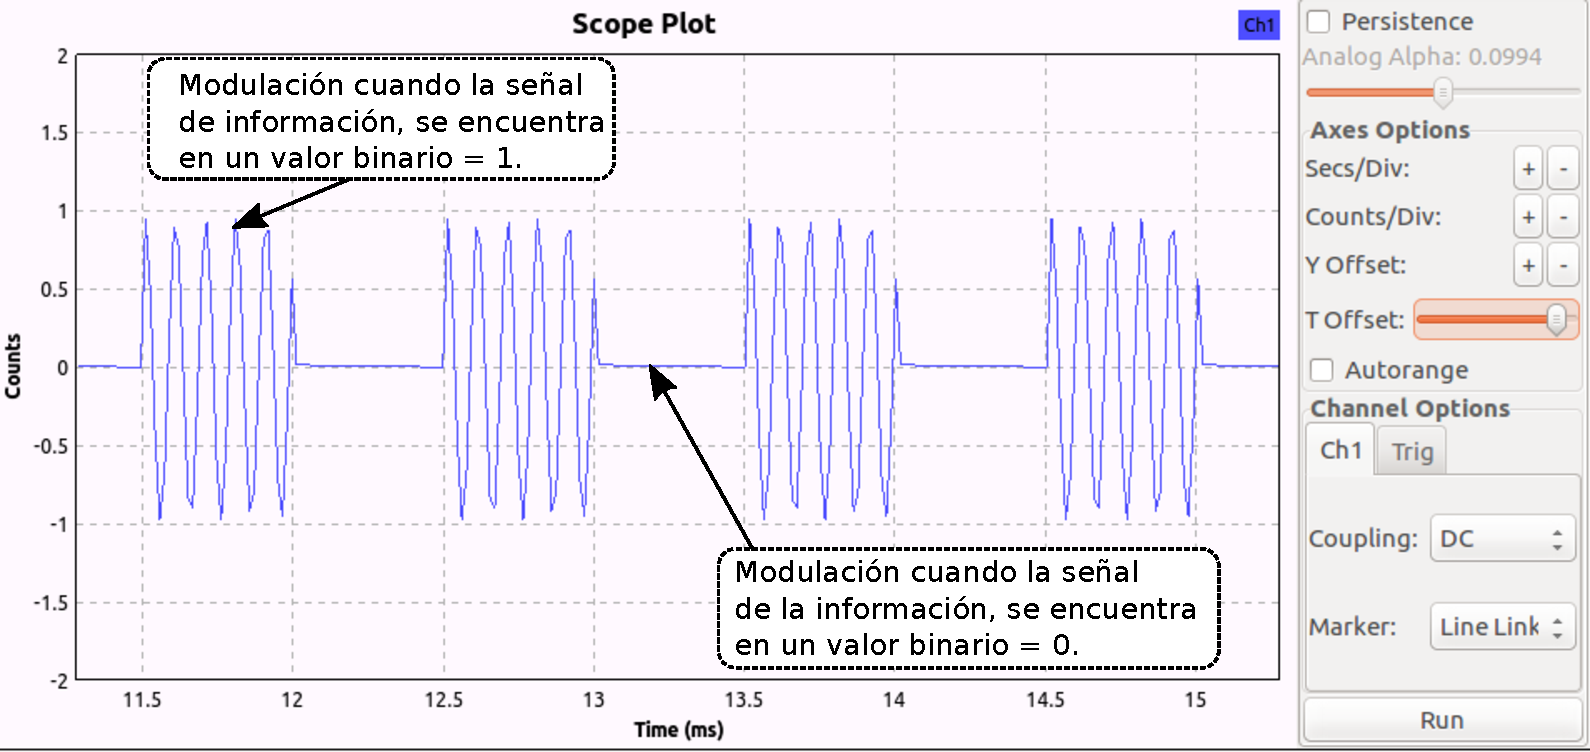
\includegraphics[width=1.1\textwidth]{parte1/lab4/pdf/lab4_3.pdf}
\end{figure}
\end{frame}
%_---------------------

\begin{frame}{Modulación ASK en GRC}

  \begin{itemize}
  \item {
La Modulación por desplazamiento de frecuencia (FSK) es una técnica de modulación digital, utilizada para la transmisión de datos. Para BFSK que corresponde al mismo proceso, pero con datos binarios, se utilizan dos frecuencias diferentes para transmitir dos señales, es decir 0 y 1. como se puede ver a continuación:

\begin{equation*}
S_{1}(t) = Acos(w_{1}t)
\end{equation*}

\begin{equation*}
S_{2}(t) = Acos(w_{2}t)
\end{equation*}

  }
  \item {
El diagrama de boques en GRC se utilizaron dos señales coseno como portadora de amplitud 1, y frecuencias de 1Khz y 10Khz. La señal 1 es representada por una onda cuadrada, y la señal 0 es obtenida restándole 1 a la señal cuadrada. Posteriormente se multiplican las señales 0 y 1 con las portadoras y luego se suman obteniendo la modulación FSK.
  }
  \end{itemize}
\end{frame}
%---------------------------


\begin{frame}{Modulación ASK en GRC}
\vspace{-8mm}
\begin{figure}[H]
\centering
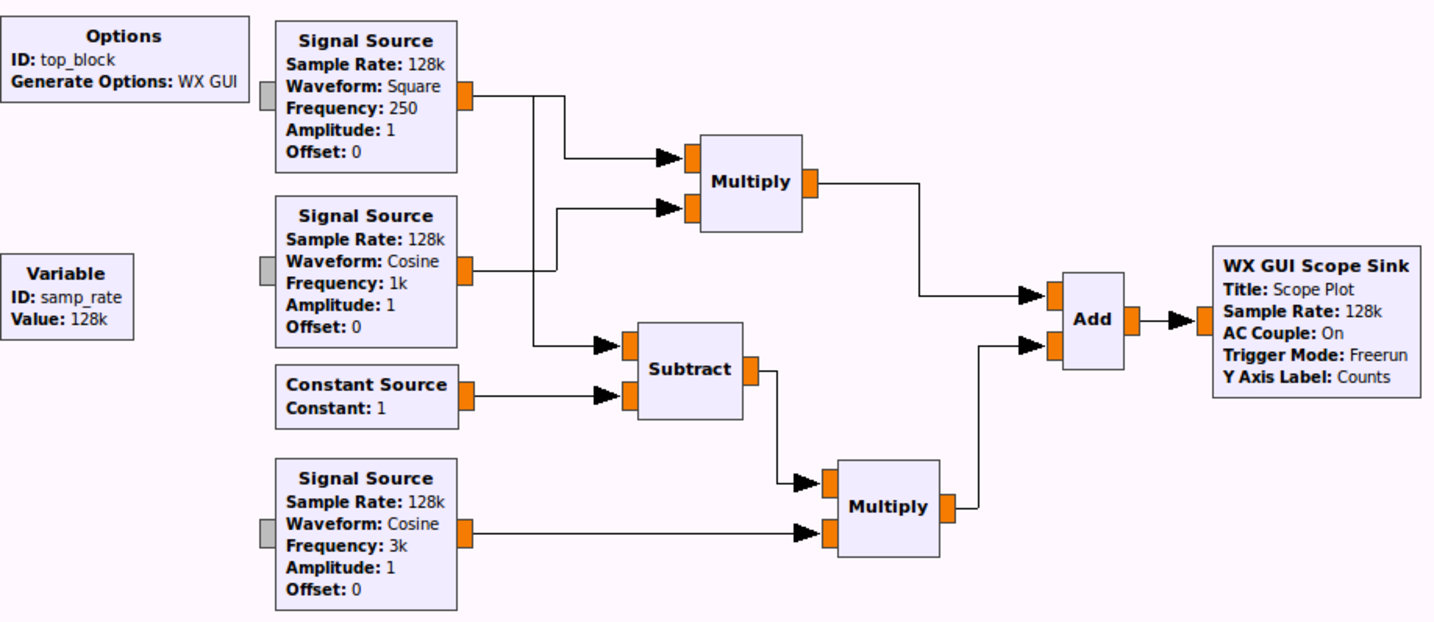
\includegraphics[width=\textwidth]{parte1/lab4/pdf/lab4_4.pdf}
\end{figure}
\end{frame}
%_---------------------

\begin{frame}{Modulación ASK en GRC}
\begin{figure}[H]
\centering
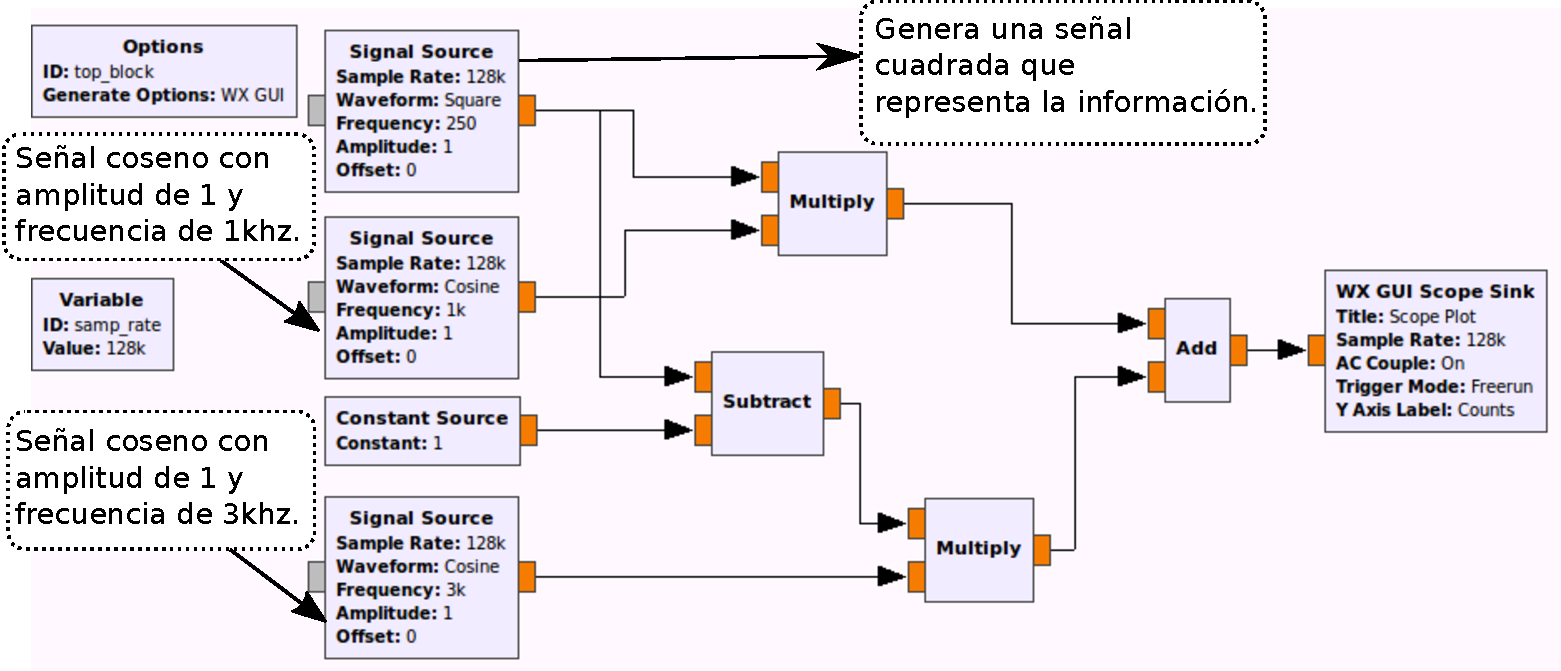
\includegraphics[width=\textwidth]{parte1/lab4/pdf/lab4_5.pdf}
\end{figure}
\end{frame}
%_---------------------

\begin{frame}{Modulación ASK en GRC}
\begin{figure}[H]
\centering
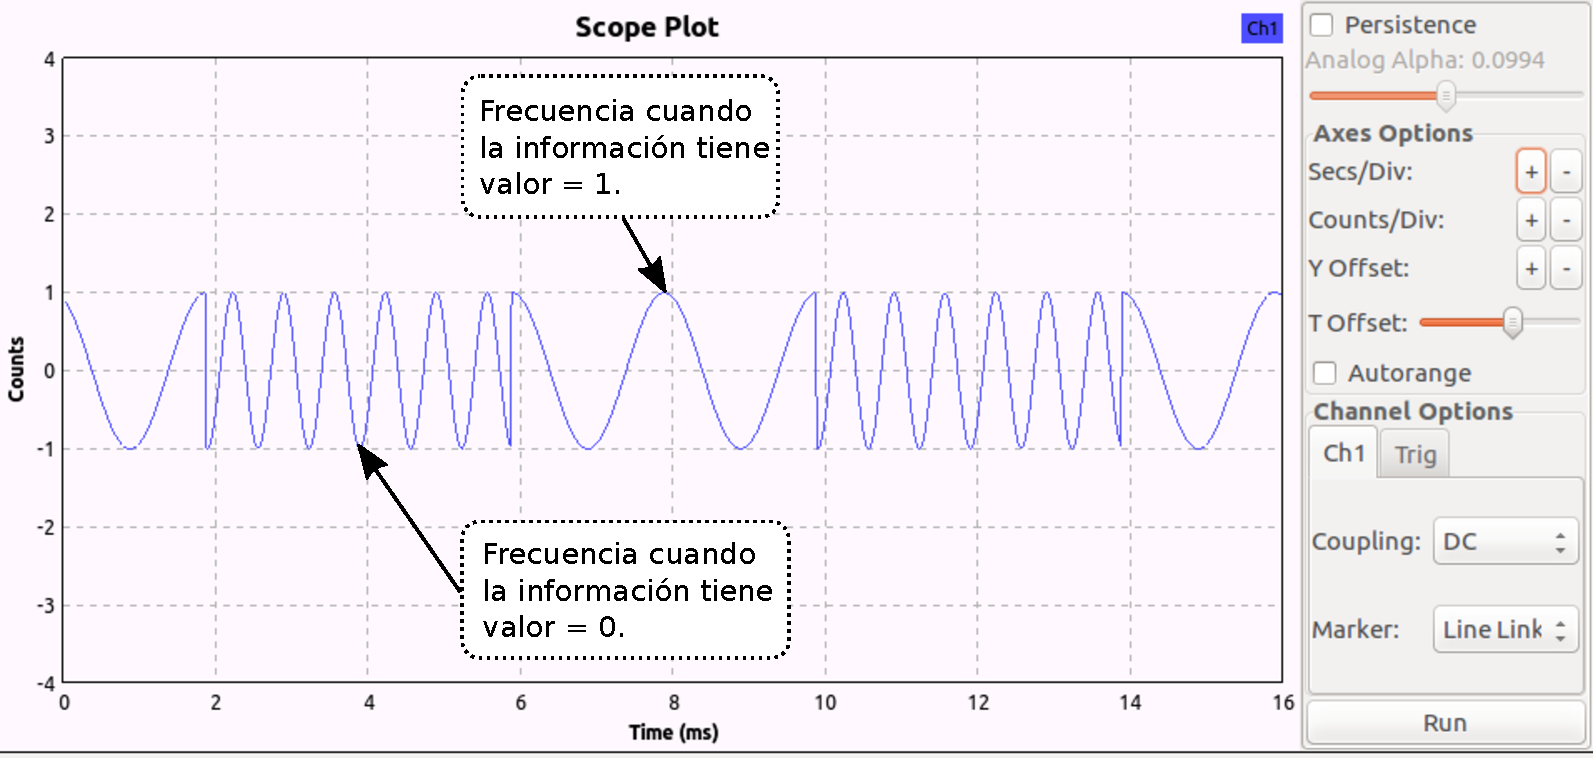
\includegraphics[width=\textwidth]{parte1/lab4/pdf/lab4_6.pdf}
\end{figure}
\end{frame}
%_---------------------

\begin{frame}{Modulacion ASK en GRC}

  \begin{itemize}
  \item {
La Modulación por desplazamiento de fase (PSK) es un esquema de modulación digital donde se varía la fase de la señal, manteniendo la frecuencia y la amplitud constante. Para la modulación PSK se usan dos señales con fases diferentes y frecuencias iguales, estas se multiplican con la señal 0 o 1 de los datos como se muestra a continuación:

\begin{equation*}
S_{1}(t) = Acos(wt)
\end{equation*}

\begin{equation*}
S_{2}(t) = Acos(wt)
\end{equation*}

  }
  \item {
El diagrama de boques en GRC se utiliza una señal coseno de 50000 Hz y la amplitud pico de 1, y otra onda sinusoidal de igual frecuencias y amplitud. Similar a BFSK se representa la señal 1 con la onda cuadrada de frecuencia 5000 Hz y el 0 por la resta de la constante.
  }
  \end{itemize}
\end{frame}
%---------------------------

\begin{frame}{Modulación ASK en GRC}
\begin{figure}[H]
\centering
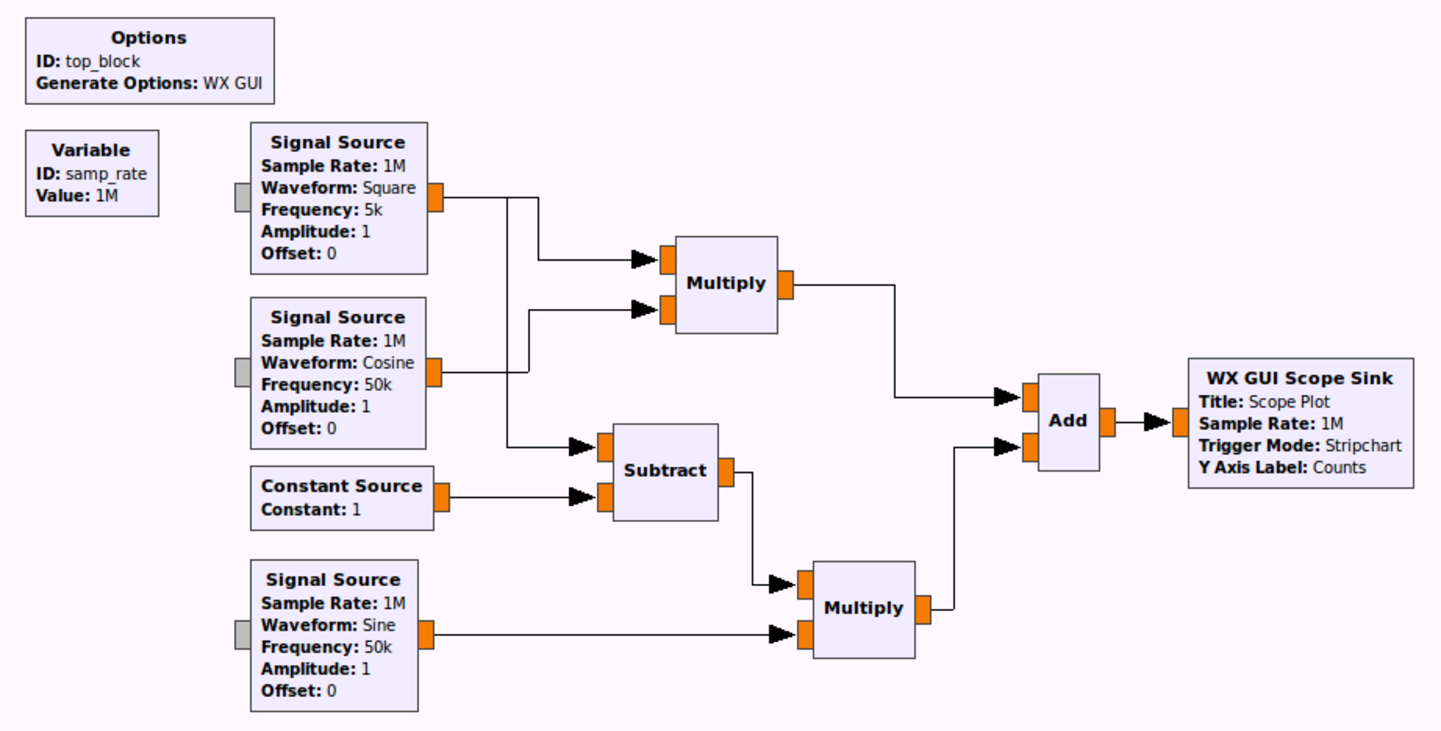
\includegraphics[width=\textwidth]{parte1/lab4/pdf/lab4_7.pdf}
\end{figure}
\end{frame}
%_---------------------

\begin{frame}{Modulación ASK en GRC}
\begin{figure}[H]
\centering
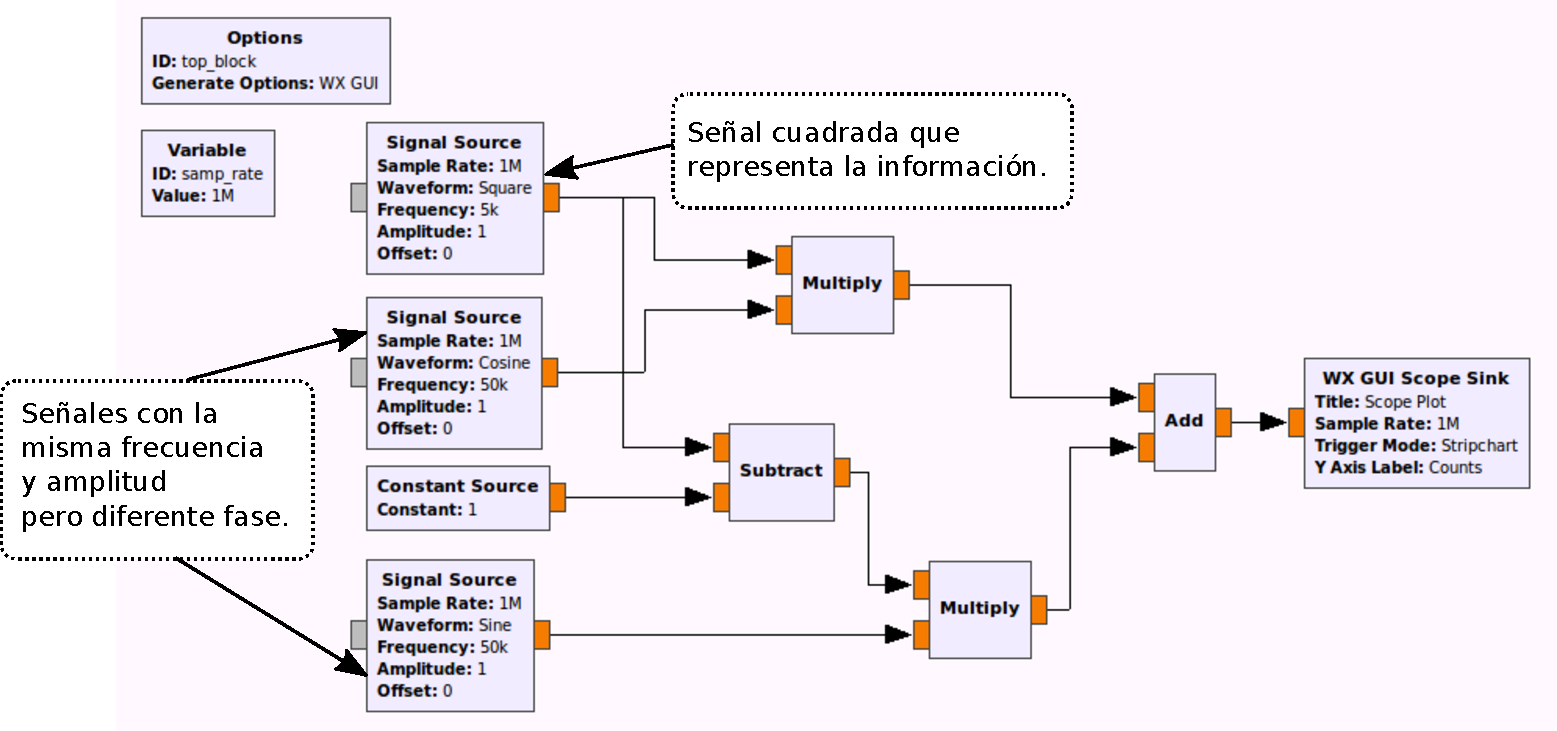
\includegraphics[width=\textwidth]{parte1/lab4/pdf/lab4_8.pdf}
\end{figure}
\end{frame}
%_---------------------
\begin{frame}{Modulación ASK en GRC}
\begin{figure}[H]
\centering
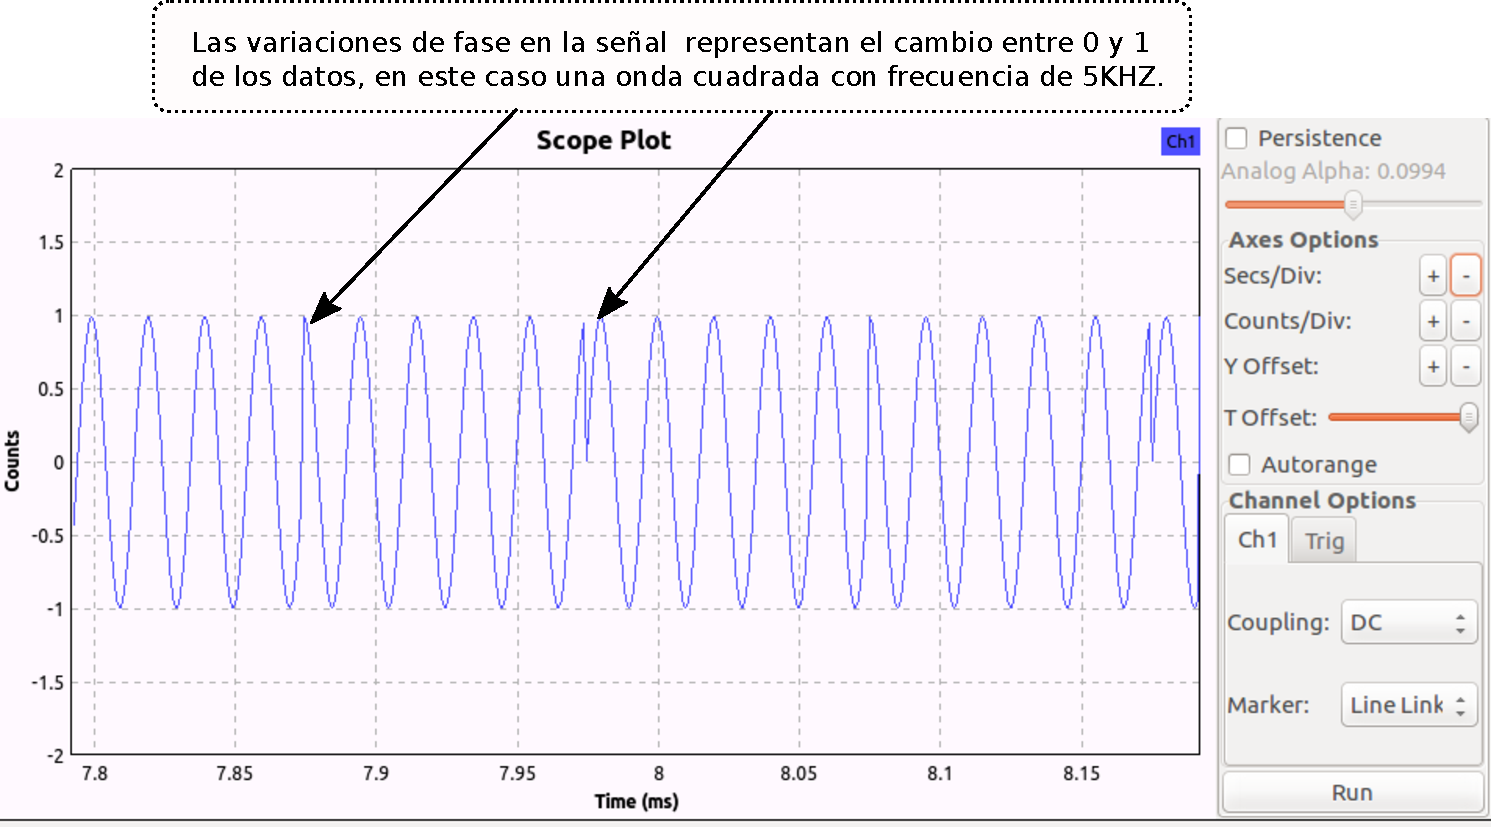
\includegraphics[width=\textwidth]{parte1/lab4/pdf/lab4_9.pdf}
\end{figure}
\end{frame}
%_---------------------